\documentclass{article}
\usepackage[pdftex]{graphicx}
\usepackage{verbatim}
\begin{document}

\author{Jon Robison}
\title{CS595 Assignment 2}
\maketitle

Q1. Write a Python program that extracts 1000 unique links from Twitter \\
See Appendix A for python program \\
See Appendix B for 1000 unique links
\\*

Q2. Download the TimeMaps for each of the target URIs... Create a histogram of
URIs vs. number of Mementos. \\
See Appendix C for python program \\
\graphicspath{{q2/}}
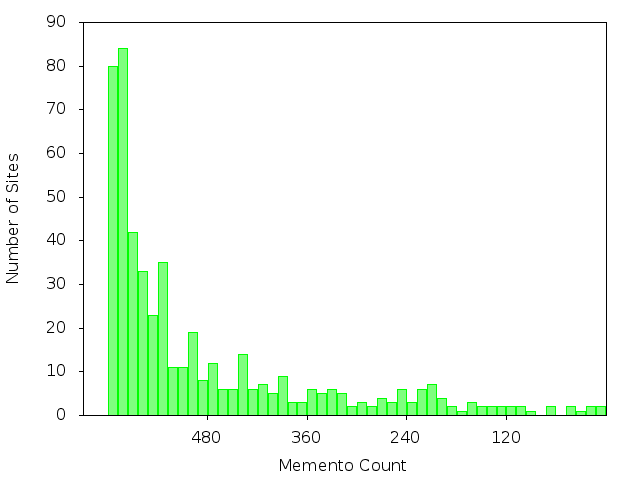
\includegraphics[scale=.4]{histogram.png}
\\*

Q3. Estimate the age of each of the 1000 URIs using the "Carbon Date" tool...
For URIs that have > 0 Mementos and an estimated creation date, create a graph
with age (in days) on one axis and number of mementos on the other. \\
See Appendix D for python program \\
\graphicspath{{q3/}}
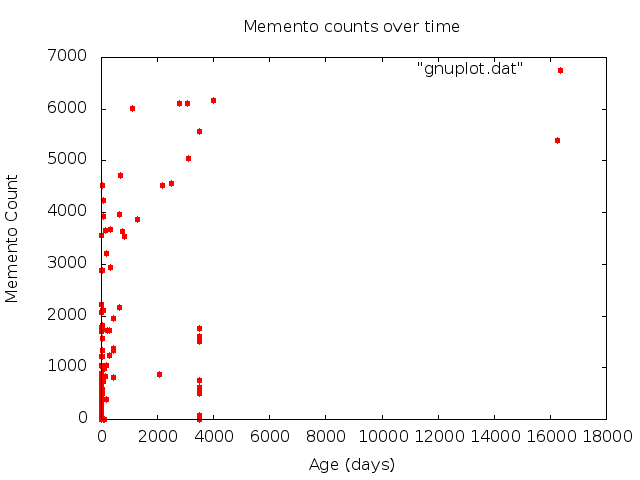
\includegraphics[scale=.4]{ageMementoCount.png}

\newpage
\appendix
Appendix A
\verbatiminput{q1/tweets.py}%

\newpage
Appendix B
\verbatiminput{q1/links.txt}%

\end{document} 
